\documentclass[12pt,a4paper]{article}

% Packages
\usepackage[utf8]{inputenc}
\usepackage[T1]{fontenc}
\usepackage{geometry}
\usepackage{graphicx}
\usepackage{hyperref}
\usepackage{enumitem}
\usepackage{xcolor}
\usepackage{tikz}
\usepackage{booktabs}
\usepackage{fancyhdr}
\usepackage{tcolorbox}
\usepackage{amsmath}
\usepackage{amssymb}

% Page geometry
\geometry{margin=2.5cm}

% Colors
\definecolor{primaryblue}{RGB}{0, 102, 204}
\definecolor{successgreen}{RGB}{40, 167, 69}
\definecolor{dangerred}{RGB}{220, 53, 69}
\definecolor{warningyellow}{RGB}{255, 193, 7}
\definecolor{lightgray}{RGB}{248, 249, 250}

% TikZ libraries
\usetikzlibrary{shapes, arrows, positioning, fit, backgrounds, calc}

% Header and footer
\pagestyle{fancy}
\fancyhf{}
\fancyhead[L]{\textbf{Software Development Project}}
\fancyhead[R]{Introduction}
\fancyfoot[C]{\thepage}

% Tcolorbox styles
\tcbuselibrary{skins, breakable}

\newtcolorbox{keyinsight}{
    colback=primaryblue!10,
    colframe=primaryblue,
    title=\textbf{Key Insight},
    fonttitle=\bfseries,
    breakable
}

\newtcolorbox{goodexample}{
    colback=successgreen!10,
    colframe=successgreen,
    title=\textbf{Good Example} \checkmark,
    fonttitle=\bfseries,
    breakable
}

\newtcolorbox{badexample}{
    colback=dangerred!10,
    colframe=dangerred,
    title=\textbf{Bad Example} $\times$,
    fonttitle=\bfseries,
    breakable
}

\newtcolorbox{definitionbox}{
    colback=lightgray,
    colframe=black!50,
    breakable
}

% Title
\title{
    \vspace{-1cm}
    \textbf{Introduction to Software Development Projects}\\
    \large Lecture Notes\\[0.5cm]
    \normalsize School of Computing Communication and Media Studies
}
\author{Masoud Hamad}
\date{CS2113 -- Software Development Project\\Academic Year 2025}

\begin{document}

\maketitle

\tableofcontents
\newpage

%============================================================
\section{What Makes a Software Development Project?}
%============================================================

Software projects emerge when there's an \textbf{identified need} and \textbf{funding}. Projects vary in duration from months to years and involve \textbf{stakeholders}---all people affected by the software, including end users and funding customers.

\begin{keyinsight}
Modern software development increasingly requires understanding stakeholder needs alongside technical skills. Research indicates most development problems are \textbf{non-technical} rather than technical in nature.
\end{keyinsight}

\subsection{Development Team Structure}

Development teams are diverse, self-organized groups (typically under 10 people) that include:

\begin{itemize}
    \item Product Owners
    \item UX/UI Designers
    \item Project Managers
    \item QA Engineers
    \item Developers
\end{itemize}

These teams follow a common \textbf{software development process} to work efficiently.

%------------------------------------------------------------
% Figure 1: Development Team Structure
%------------------------------------------------------------
\begin{figure}[htbp]
\centering
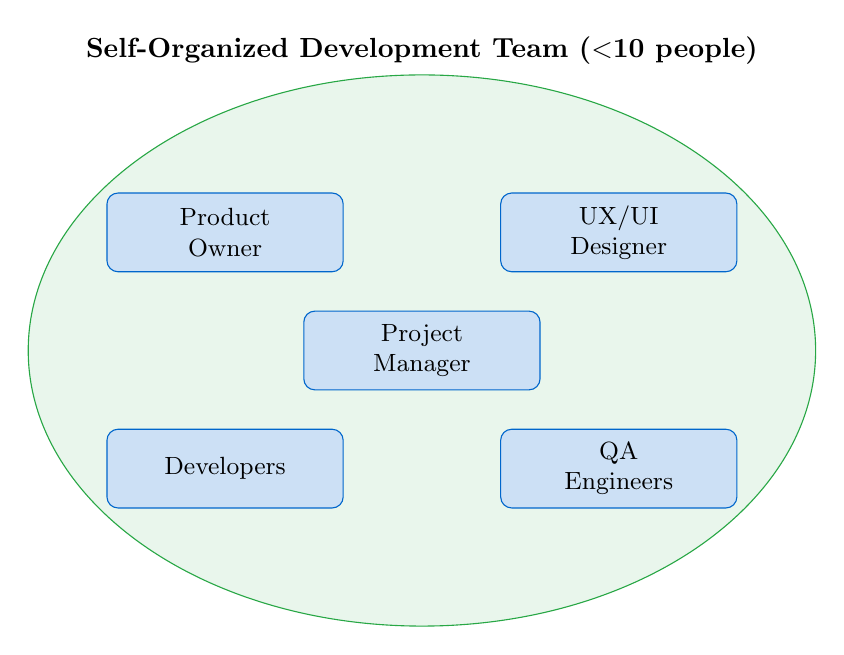
\begin{tikzpicture}[
    node distance=1.5cm,
    role/.style={rectangle, draw=primaryblue, fill=primaryblue!20, rounded corners, minimum width=3cm, minimum height=1cm, align=center, font=\small},
    team/.style={ellipse, draw=successgreen, fill=successgreen!10, minimum width=4cm, minimum height=2cm}
]
    % Team circle
    \node[team, minimum width=10cm, minimum height=7cm] (team) {};
    \node[above] at (team.north) {\textbf{Self-Organized Development Team ($<$10 people)}};

    % Roles
    \node[role] (po) at (-2.5, 1.5) {Product\\Owner};
    \node[role] (ux) at (2.5, 1.5) {UX/UI\\Designer};
    \node[role] (pm) at (0, 0) {Project\\Manager};
    \node[role] (dev) at (-2.5, -1.5) {Developers};
    \node[role] (qa) at (2.5, -1.5) {QA\\Engineers};

\end{tikzpicture}
\caption{Typical Software Development Team Structure}
\label{fig:team-structure}
\end{figure}

%============================================================
\section{Agile Principles in Software Development}
%============================================================

The \textbf{Manifesto for Agile Software Development} emphasizes:

\begin{tcolorbox}[colback=primaryblue!5, colframe=primaryblue, title=\textbf{Agile Manifesto Values}]
\begin{enumerate}
    \item \textbf{Individuals and interactions} over processes and tools
    \item \textbf{Working software} over comprehensive documentation
    \item \textbf{Customer collaboration} over contract negotiation
    \item \textbf{Responding to change} over following a plan
\end{enumerate}
\end{tcolorbox}

\begin{keyinsight}
A critical agile value is \textbf{welcoming change}, since requirements frequently shift during development. The Manifesto doesn't specify implementation details; frameworks like \textbf{Scrum} and \textbf{SAFe} provide concrete processes.
\end{keyinsight}

%============================================================
\section{Software Development Lifecycle (SDLC)}
%============================================================

Six phases structure development:

\subsection{The Six Phases}

\begin{enumerate}
    \item \textbf{Requirements Phase:} Collecting stakeholder needs into a software requirement specification document

    \item \textbf{Design Phase:} Analyzing requirements and identifying solutions

    \item \textbf{Implementation Phase:} Developers code daily tasks toward final product

    \item \textbf{Test Phase:} Combining automation and manual testing to identify bugs

    \item \textbf{Deployment Phase:} Distributing software to the production environment (vs. development environment for developers)

    \item \textbf{Maintenance Phase:} Fixing bugs, addressing issues, monitoring performance
\end{enumerate}

%------------------------------------------------------------
% Figure 2: Software Development Lifecycle
%------------------------------------------------------------
\begin{figure}[htbp]
\centering
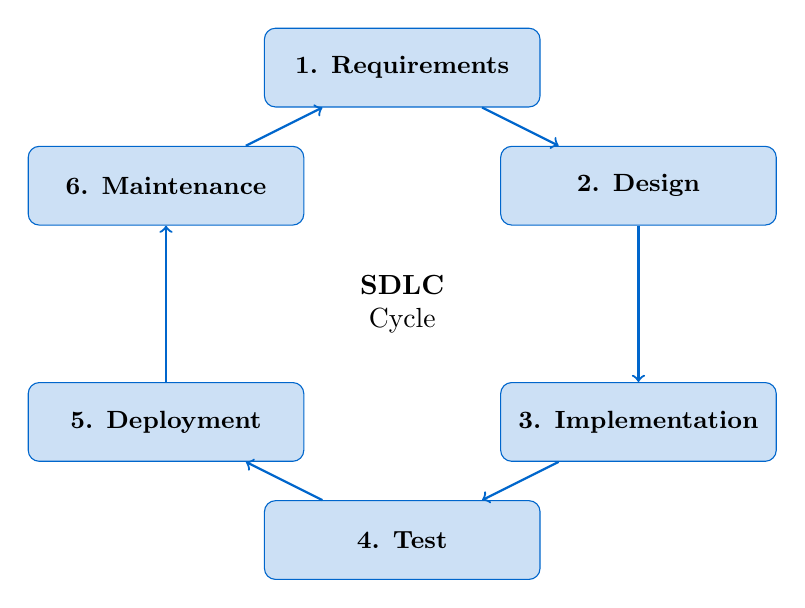
\begin{tikzpicture}[
    node distance=0.3cm,
    phase/.style={rectangle, draw=primaryblue, fill=primaryblue!20, rounded corners, minimum width=3.5cm, minimum height=1cm, align=center, font=\small\bfseries},
    arrow/.style={->, thick, primaryblue}
]
    % Phases in a cycle
    \node[phase] (req) at (0,3) {1. Requirements};
    \node[phase] (des) at (3,1.5) {2. Design};
    \node[phase] (imp) at (3,-1.5) {3. Implementation};
    \node[phase] (test) at (0,-3) {4. Test};
    \node[phase] (dep) at (-3,-1.5) {5. Deployment};
    \node[phase] (maint) at (-3,1.5) {6. Maintenance};

    % Arrows
    \draw[arrow] (req) -- (des);
    \draw[arrow] (des) -- (imp);
    \draw[arrow] (imp) -- (test);
    \draw[arrow] (test) -- (dep);
    \draw[arrow] (dep) -- (maint);
    \draw[arrow] (maint) -- (req);

    % Center label
    \node[align=center] at (0,0) {\textbf{SDLC}\\Cycle};

\end{tikzpicture}
\caption{Software Development Lifecycle Phases}
\label{fig:sdlc}
\end{figure}

\subsection{Waterfall Model}

\begin{definitionbox}
\textbf{Waterfall Model:} A traditional sequential approach completing each phase before the next begins. This approach required all requirements upfront and prevented mid-project changes.
\end{definitionbox}

\textbf{Problem:} This approach is problematic because requirements \textit{inevitably shift} during development.

%------------------------------------------------------------
% Figure 3: Waterfall vs Agile
%------------------------------------------------------------
\begin{figure}[htbp]
\centering
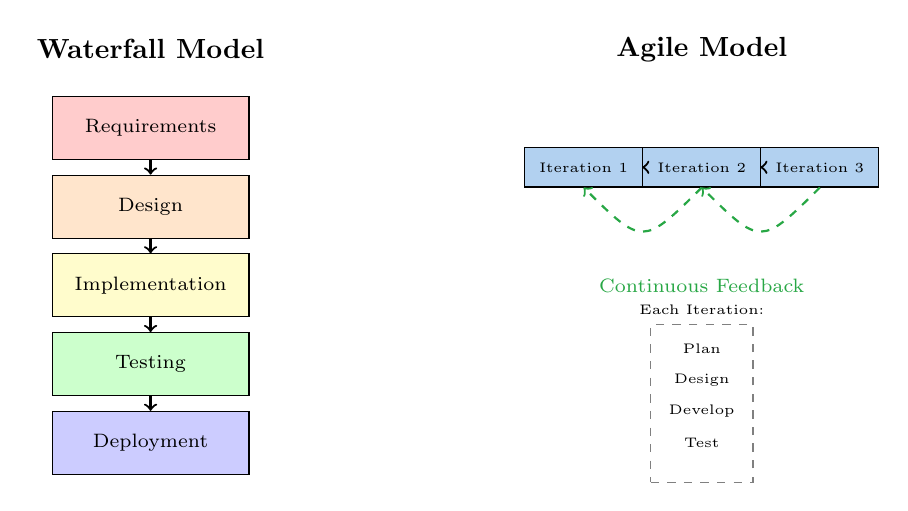
\begin{tikzpicture}[
    node distance=0.5cm,
    phase/.style={rectangle, draw, fill=gray!20, minimum width=2.5cm, minimum height=0.8cm, align=center, font=\scriptsize},
    arrow/.style={->, thick}
]
    % Waterfall side
    \node[font=\bfseries] at (-4, 3) {Waterfall Model};
    \node[phase, fill=red!20] (w1) at (-4, 2) {Requirements};
    \node[phase, fill=orange!20] (w2) at (-4, 1) {Design};
    \node[phase, fill=yellow!20] (w3) at (-4, 0) {Implementation};
    \node[phase, fill=green!20] (w4) at (-4, -1) {Testing};
    \node[phase, fill=blue!20] (w5) at (-4, -2) {Deployment};

    \draw[arrow] (w1) -- (w2);
    \draw[arrow] (w2) -- (w3);
    \draw[arrow] (w3) -- (w4);
    \draw[arrow] (w4) -- (w5);

    % Agile side
    \node[font=\bfseries] at (3, 3) {Agile Model};

    % Iteration 1
    \node[phase, fill=primaryblue!30, minimum width=1.5cm, minimum height=0.5cm] (a1) at (1.5, 1.5) {\tiny Iteration 1};
    \node[phase, fill=primaryblue!30, minimum width=1.5cm, minimum height=0.5cm] (a2) at (3, 1.5) {\tiny Iteration 2};
    \node[phase, fill=primaryblue!30, minimum width=1.5cm, minimum height=0.5cm] (a3) at (4.5, 1.5) {\tiny Iteration 3};

    \draw[arrow] (a1) -- (a2);
    \draw[arrow] (a2) -- (a3);

    % Feedback loops
    \draw[arrow, dashed, successgreen] (a2.south) .. controls (2.25, 0.5) .. (a1.south);
    \draw[arrow, dashed, successgreen] (a3.south) .. controls (3.75, 0.5) .. (a2.south);

    \node[font=\scriptsize, successgreen] at (3, 0) {Continuous Feedback};

    % Each iteration contains
    \node[rectangle, draw=gray, dashed, minimum width=1.3cm, minimum height=2cm] (iter) at (3, -1.5) {};
    \node[font=\tiny, above] at (iter.north) {Each Iteration:};
    \node[font=\tiny] at (3, -0.8) {Plan};
    \node[font=\tiny] at (3, -1.2) {Design};
    \node[font=\tiny] at (3, -1.6) {Develop};
    \node[font=\tiny] at (3, -2.0) {Test};

\end{tikzpicture}
\caption{Comparison: Waterfall vs Agile Development Models}
\label{fig:waterfall-vs-agile}
\end{figure}

%============================================================
\section{Agile Software Development Process}
%============================================================

Agile uses \textbf{iterative approaches} with short iterations (one to two weeks). Each iteration specifies only necessary requirements, allowing flexibility.

\begin{keyinsight}
Teams implement requirements, producing \textbf{working software} users can test and provide feedback on---creating a \textbf{feedback loop} essential to agile processes.
\end{keyinsight}

Unlike sequential phases, agile completes \textbf{all lifecycle phases within each iteration cycle}. This repeating cycle accommodates continuous improvement.

%------------------------------------------------------------
% Figure 4: Agile Iteration Cycle
%------------------------------------------------------------
\begin{figure}[htbp]
\centering
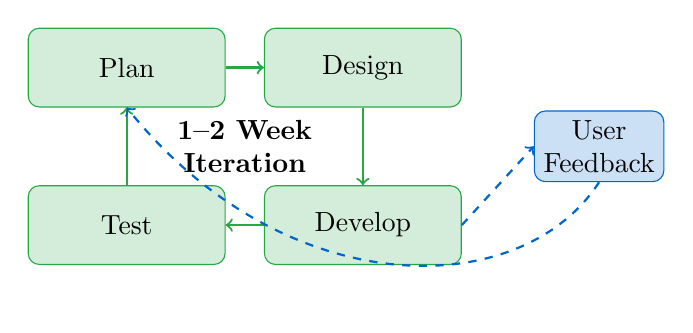
\begin{tikzpicture}[
    node distance=1cm,
    block/.style={rectangle, draw=successgreen, fill=successgreen!20, rounded corners, minimum width=2.5cm, minimum height=1cm, align=center},
    arrow/.style={->, thick, successgreen}
]
    % Iteration cycle
    \node[block] (plan) at (0, 2) {Plan};
    \node[block] (design) at (3, 2) {Design};
    \node[block] (develop) at (3, 0) {Develop};
    \node[block] (test) at (0, 0) {Test};

    \draw[arrow] (plan) -- (design);
    \draw[arrow] (design) -- (develop);
    \draw[arrow] (develop) -- (test);
    \draw[arrow] (test) -- (plan);

    % Center
    \node[align=center, font=\bfseries] at (1.5, 1) {1--2 Week\\Iteration};

    % User feedback
    \node[rectangle, draw=primaryblue, fill=primaryblue!20, rounded corners, align=center] (user) at (6, 1) {User\\Feedback};
    \draw[arrow, primaryblue, dashed] (develop.east) -- (user.west);
    \draw[arrow, primaryblue, dashed] (user.south) .. controls (5, -1) and (2, -1) .. (plan.south);

\end{tikzpicture}
\caption{Agile Iteration Cycle with User Feedback Loop}
\label{fig:agile-cycle}
\end{figure}

%============================================================
\section{Scrum Framework}
%============================================================

\begin{definitionbox}
\textbf{Scrum} is the most widely adopted agile framework (\textbf{87\%} of respondents in 2022 State of Agile report). The Scrum Guide is the official reference.
\end{definitionbox}

The framework defines:
\begin{itemize}
    \item \textbf{Roles} (Scrum Master, Product Owner, Developers)
    \item \textbf{Events} (Sprint, Sprint Planning, Daily Scrum, Sprint Review, Sprint Retrospective)
    \item \textbf{Artifacts} (Product Backlog, Sprint Backlog, Increment)
\end{itemize}

%------------------------------------------------------------
% Figure 5: Scrum Framework Overview
%------------------------------------------------------------
\begin{figure}[htbp]
\centering
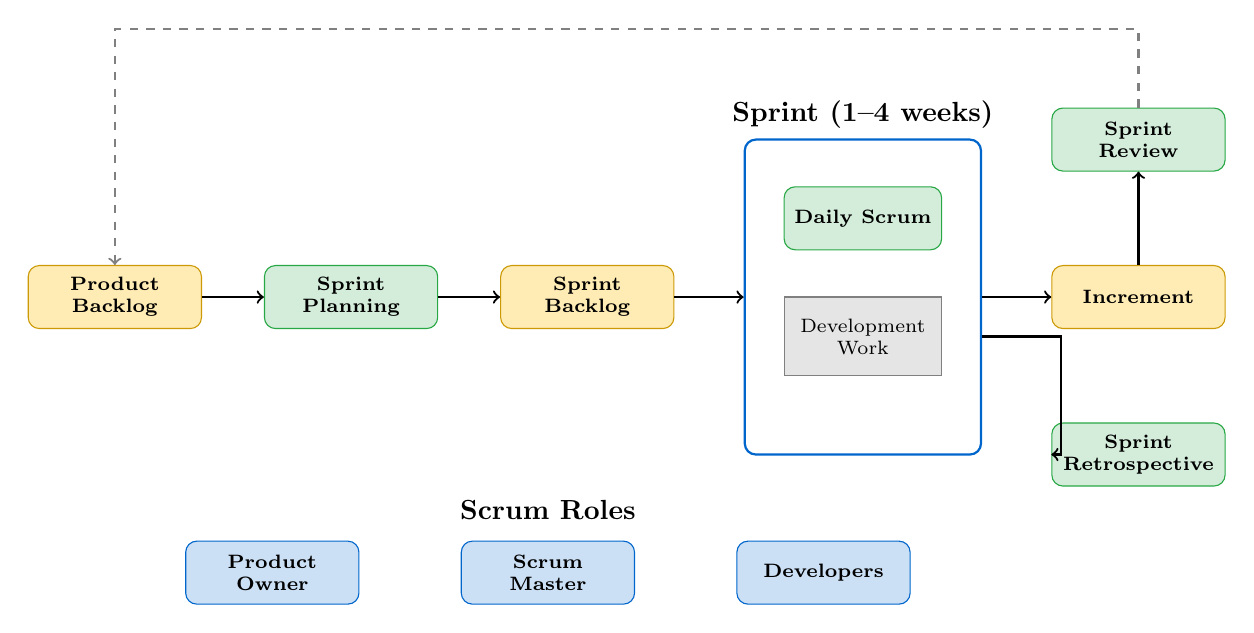
\begin{tikzpicture}[
    node distance=0.8cm,
    role/.style={rectangle, draw=primaryblue, fill=primaryblue!20, rounded corners, minimum width=2.2cm, minimum height=0.8cm, align=center, font=\scriptsize\bfseries},
    event/.style={rectangle, draw=successgreen, fill=successgreen!20, rounded corners, minimum width=2.2cm, minimum height=0.8cm, align=center, font=\scriptsize\bfseries},
    artifact/.style={rectangle, draw=warningyellow!80!black, fill=warningyellow!30, rounded corners, minimum width=2.2cm, minimum height=0.8cm, align=center, font=\scriptsize\bfseries},
    arrow/.style={->, thick}
]
    % Product Backlog
    \node[artifact] (pb) at (-4, 0) {Product\\Backlog};

    % Sprint Planning
    \node[event] (sp) at (-1, 0) {Sprint\\Planning};

    % Sprint Backlog
    \node[artifact] (sb) at (2, 0) {Sprint\\Backlog};

    % Sprint (main cycle)
    \node[rectangle, draw=primaryblue, thick, minimum width=3cm, minimum height=4cm, rounded corners] (sprint) at (5.5, 0) {};
    \node[font=\bfseries, above] at (sprint.north) {Sprint (1--4 weeks)};

    % Daily Scrum inside sprint
    \node[event, minimum width=2cm] (ds) at (5.5, 1) {Daily Scrum};

    % Development work
    \node[rectangle, draw=gray, fill=gray!20, minimum width=2cm, minimum height=1cm, align=center, font=\scriptsize] (dev) at (5.5, -0.5) {Development\\Work};

    % Increment
    \node[artifact] (inc) at (9, 0) {Increment};

    % Sprint Review and Retro
    \node[event] (sr) at (9, 2) {Sprint\\Review};
    \node[event] (retro) at (9, -2) {Sprint\\Retrospective};

    % Arrows
    \draw[arrow] (pb) -- (sp);
    \draw[arrow] (sp) -- (sb);
    \draw[arrow] (sb) -- (sprint.west);
    \draw[arrow] (sprint.east) -- (inc);
    \draw[arrow] (inc) -- (sr);
    \draw[arrow] (sprint.east) ++ (0, -0.5) -- ++ (1, 0) |- (retro);

    % Feedback to backlog
    \draw[arrow, dashed, gray] (sr.north) |- ++ (-6, 1) -| (pb.north);

    % Roles at bottom
    \node[role] (po) at (-2, -3.5) {Product\\Owner};
    \node[role] (sm) at (1.5, -3.5) {Scrum\\Master};
    \node[role] (devs) at (5, -3.5) {Developers};

    \node[font=\bfseries] at (1.5, -2.7) {Scrum Roles};

\end{tikzpicture}
\caption{Scrum Framework Overview}
\label{fig:scrum-framework}
\end{figure}

%============================================================
\section{Requirement Categories}
%============================================================

Requirements divide into two types:

\subsection{Functional Requirements}

\begin{definitionbox}
\textbf{Functional Requirements:} User-visible features that describe what the system should do.
\end{definitionbox}

\textbf{Examples:}
\begin{itemize}
    \item ``User should register with username and password''
    \item ``User should see latest blog posts from favorite blogs''
\end{itemize}

\subsection{Non-Functional Requirements}

\begin{definitionbox}
\textbf{Non-Functional Requirements:} Quality constraints invisible to users but addressing security, performance, etc.
\end{definitionbox}

\textbf{Examples:}
\begin{itemize}
    \item ``Passwords stored as Bcrypt hashes''
    \item ``Blog post lists load in under one second average''
\end{itemize}

%------------------------------------------------------------
% Figure 6: Requirement Categories
%------------------------------------------------------------
\begin{figure}[htbp]
\centering
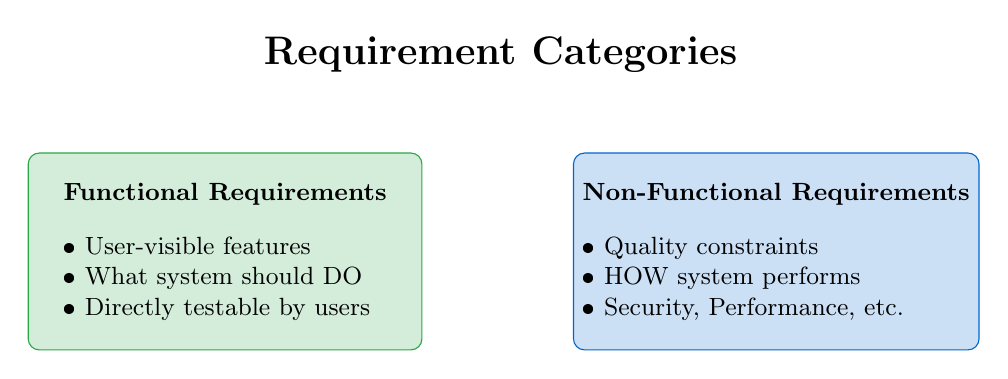
\begin{tikzpicture}[
    node distance=1cm,
    box/.style={rectangle, draw, rounded corners, minimum width=5cm, minimum height=2.5cm, align=left, font=\small},
]
    % Functional
    \node[box, fill=successgreen!20, draw=successgreen] (func) at (-3.5, 0) {
        \textbf{Functional Requirements}\\[0.3cm]
        \textbullet\ User-visible features\\
        \textbullet\ What system should DO\\
        \textbullet\ Directly testable by users
    };

    % Non-functional
    \node[box, fill=primaryblue!20, draw=primaryblue] (nfunc) at (3.5, 0) {
        \textbf{Non-Functional Requirements}\\[0.3cm]
        \textbullet\ Quality constraints\\
        \textbullet\ HOW system performs\\
        \textbullet\ Security, Performance, etc.
    };

    % Header
    \node[font=\Large\bfseries] at (0, 2.5) {Requirement Categories};

\end{tikzpicture}
\caption{Functional vs Non-Functional Requirements}
\label{fig:requirements}
\end{figure}

%============================================================
\section{User Stories}
%============================================================

In agile development, functional requirements become \textbf{user stories}---short descriptions from the user's perspective. Each sprint, developers implement features based on user stories.

\subsection{Standard Format}

\begin{tcolorbox}[colback=primaryblue!10, colframe=primaryblue, title=\textbf{User Story Template}]
\centering
\Large
``As a \textbf{[user persona]}, I want \textbf{[action]} so that \textbf{[goal]}.''
\end{tcolorbox}

\subsection{Examples}

\begin{goodexample}
\begin{itemize}
    \item ``As a \textbf{content creator}, I want to \textbf{create blogs} so I can \textbf{write posts for readers}.''
    \item ``As a \textbf{blog reader}, I want to \textbf{browse blog posts} so I can \textbf{find interesting content}.''
\end{itemize}
\end{goodexample}

\begin{keyinsight}
User stories are brief reminders of features needing implementation, written from users' perspectives \textbf{without technical details}.
\end{keyinsight}

%============================================================
\section{Writing Good User Stories: INVEST Criteria}
%============================================================

Strong user stories must:
\begin{itemize}
    \item Focus on \textbf{end-user value}
    \item Follow the \textbf{INVEST criteria}
\end{itemize}

\subsection{INVEST Criteria}

%------------------------------------------------------------
% Figure 7: INVEST Criteria
%------------------------------------------------------------
\begin{figure}[htbp]
\centering
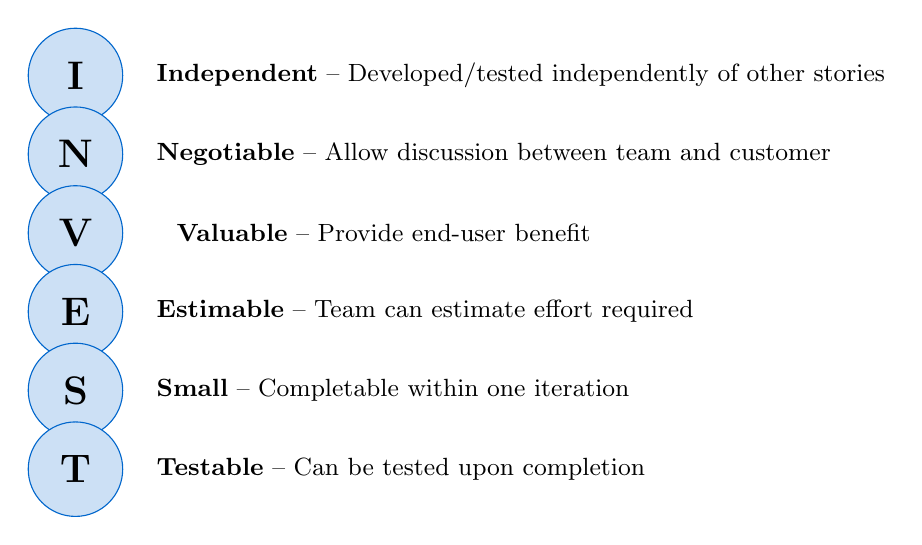
\begin{tikzpicture}[
    node distance=0.3cm,
    letter/.style={circle, draw=primaryblue, fill=primaryblue!20, minimum size=1.2cm, font=\Large\bfseries},
    desc/.style={rectangle, minimum width=6cm, align=left, font=\small}
]
    \node[letter] (i) at (0, 5) {I};
    \node[desc, right=of i] {\textbf{Independent} -- Developed/tested independently of other stories};

    \node[letter] (n) at (0, 4) {N};
    \node[desc, right=of n] {\textbf{Negotiable} -- Allow discussion between team and customer};

    \node[letter] (v) at (0, 3) {V};
    \node[desc, right=of v] {\textbf{Valuable} -- Provide end-user benefit};

    \node[letter] (e) at (0, 2) {E};
    \node[desc, right=of e] {\textbf{Estimable} -- Team can estimate effort required};

    \node[letter] (s) at (0, 1) {S};
    \node[desc, right=of s] {\textbf{Small} -- Completable within one iteration};

    \node[letter] (t) at (0, 0) {T};
    \node[desc, right=of t] {\textbf{Testable} -- Can be tested upon completion};

\end{tikzpicture}
\caption{INVEST Criteria for User Stories}
\label{fig:invest}
\end{figure}

\subsection{Common Problems and Solutions}

\subsubsection{Problem 1: Too Large (violates ``Small'')}

\begin{badexample}
``As content creator, I want to register with username, password, profile picture, and description''
\end{badexample}

\begin{goodexample}
Split into multiple stories:
\begin{itemize}
    \item Register with username/password
    \item Add profile picture
    \item Add profile description
\end{itemize}
\end{goodexample}

\subsubsection{Problem 2: Lacks Technical Clarity (violates ``Estimable'')}

\begin{badexample}
``As content creator, I want to export posts from all social media platforms''
\end{badexample}

\begin{goodexample}
Narrower scope:\\
``As content creator, I want to export posts from Medium''
\end{goodexample}

\subsubsection{Problem 3: Written from Developer Perspective}

\begin{badexample}
``As developer, I want to add database index to optimize blog posts table loading''
\end{badexample}

\begin{goodexample}
User-focused:\\
``As blog reader, I want blog post lists loading quickly to find content''
\end{goodexample}

%------------------------------------------------------------
% Figure 8: User Story Quality Checklist
%------------------------------------------------------------
\begin{figure}[htbp]
\centering
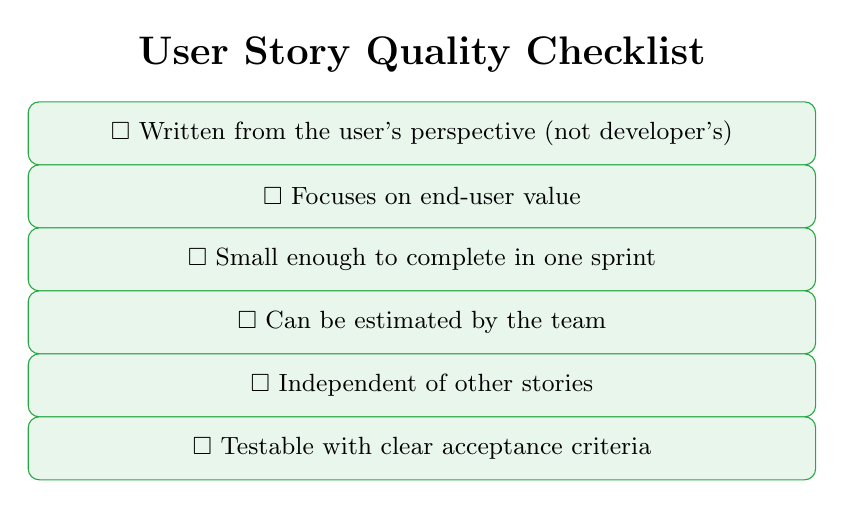
\begin{tikzpicture}[
    node distance=0.5cm,
    check/.style={rectangle, draw=successgreen, fill=successgreen!10, rounded corners, minimum width=10cm, minimum height=0.8cm, align=left, font=\small}
]
    \node[font=\Large\bfseries] at (0, 4) {User Story Quality Checklist};

    \node[check] (c1) at (0, 3) {$\square$ Written from the user's perspective (not developer's)};
    \node[check] (c2) at (0, 2.2) {$\square$ Focuses on end-user value};
    \node[check] (c3) at (0, 1.4) {$\square$ Small enough to complete in one sprint};
    \node[check] (c4) at (0, 0.6) {$\square$ Can be estimated by the team};
    \node[check] (c5) at (0, -0.2) {$\square$ Independent of other stories};
    \node[check] (c6) at (0, -1) {$\square$ Testable with clear acceptance criteria};

\end{tikzpicture}
\caption{User Story Quality Checklist}
\label{fig:checklist}
\end{figure}

%============================================================
\newpage
\section{Exercises}
%============================================================

\begin{tcolorbox}[colback=warningyellow!10, colframe=warningyellow!80!black, title=\textbf{Submission Requirements}]
Exercises must be submitted as a \textbf{single PDF} to Moodle before \textbf{Sunday, January 4, 2026}. Submission is required to confirm course participation.
\end{tcolorbox}

\vspace{0.5cm}

\subsection{Exercise 1: Scrum Team Roles}
Identify the roles in a Scrum Team and describe the responsibilities of each role.

\vspace{0.5cm}

\subsection{Exercise 2: Sprints and Scrum Events}
Explain what a Sprint is and describe the different Scrum events that occur during a Sprint.

\vspace{0.5cm}

\subsection{Exercise 3: Product Backlog vs Sprint Backlog}
What is the difference between a Product Backlog and a Sprint Backlog? Who is responsible for each?

\vspace{0.5cm}

\subsection{Exercises 4--8: Scrum Principles}
\begin{enumerate}[start=4]
    \item Discuss the three pillars of Scrum (Transparency, Inspection, Adaptation).
    \item How do the three pillars support empirical process control?
    \item Compare and contrast Scrum with the Waterfall model.
    \item What are the advantages of Scrum over Waterfall?
    \item In what situations might Waterfall be preferred over Scrum?
\end{enumerate}

\vspace{0.5cm}

\subsection{Exercise 9: True or False}
Evaluate the following statements about Scrum practices. For each, state whether it is True or False and explain your reasoning.

\begin{enumerate}[label=\alph*)]
    \item The Scrum Master assigns tasks to team members.
    \item The Product Owner can change the Sprint Backlog during the Sprint.
    \item Daily Scrum meetings should be limited to 15 minutes.
    \item The Sprint Review is the same as the Sprint Retrospective.
    \item Only developers attend the Daily Scrum.
\end{enumerate}

\vspace{0.5cm}

\subsection{Exercise 10: Critique User Stories}
The following user stories have problems. Identify what is wrong with each and explain which INVEST criterion is violated.

\begin{enumerate}[label=\alph*)]
    \item ``As a developer, I want to refactor the codebase so the code is cleaner.''
    \item ``As a user, I want the system to be fast.''
    \item ``As an admin, I want to manage users, create reports, configure settings, and monitor system health.''
    \item ``As a customer, I want to buy products from the website.''
\end{enumerate}

\vspace{0.5cm}

\subsection{Exercise 11: Improve User Stories}
Rewrite the following poorly written user stories to make them better:

\begin{enumerate}[label=\alph*)]
    \item ``The system should have a login feature.''
    \item ``As a developer, I need to add a REST API endpoint.''
    \item ``Users should be able to do everything related to their profile.''
\end{enumerate}

\vspace{0.5cm}

\subsection{Exercise 12: Create User Stories}
Based on a blogging platform project description, create \textbf{six user stories} using the proper format:

\begin{quote}
``As a [user persona], I want [action] so that [goal].''
\end{quote}

Consider different user personas such as:
\begin{itemize}
    \item Blog reader
    \item Content creator
    \item Administrator
\end{itemize}

\vspace{0.5cm}

\subsection{Exercise 13: Prioritize User Stories}
Take the six user stories you created in Exercise 12 and prioritize them. Consider:

\begin{itemize}
    \item Which stories provide the most value to users?
    \item Which stories have dependencies on other stories?
    \item Which stories should be implemented first in a Minimum Viable Product (MVP)?
\end{itemize}

Create a prioritized list and explain your reasoning for the ordering.

\vspace{0.5cm}

\subsection{Bonus Exercise: Team Formation}
Form team preferences on a collaborative board. Discuss with your classmates:
\begin{itemize}
    \item What skills do you bring to a team?
    \item What areas do you want to improve?
    \item What type of project interests you most?
\end{itemize}

%============================================================
\vspace{1cm}
\hrule
\vspace{0.3cm}
\begin{center}
\small
\textit{This document is licensed under Creative Commons BY-NC-SA 4.0}
\end{center}

\end{document}
